% TikZ Variables and Calculations
% Demonstrates: \def, \pgfmathsetmacro, foreach loops, and coordinate math.
% Compile with: pdflatex main.tex

\documentclass{article}
\usepackage{tikz}
\usetikzlibrary{calc}

\begin{document}
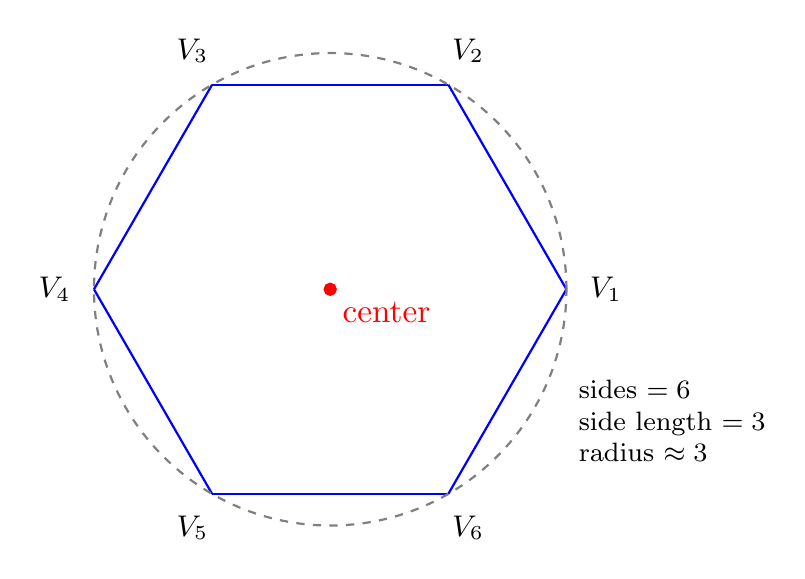
\begin{tikzpicture}[thick, scale=1, every node/.style={scale=1.2}]

% --- Define variables with \def ---
\def\sideLength{3}
\def\numSides{6}

% --- Calculate derived values with \pgfmathsetmacro ---
\pgfmathsetmacro{\angle}{360/\numSides}
\pgfmathsetmacro{\radius}{\sideLength / (2 * sin(\angle/2))}

% --- Draw a regular polygon using variables and a loop ---
\foreach \i in {1,...,\numSides} {
    \pgfmathsetmacro{\startAngle}{\angle * (\i - 1)}
    \pgfmathsetmacro{\endAngle}{\angle * \i}
    \draw[blue, thick]
        ({\radius * cos(\startAngle)}, {\radius * sin(\startAngle)})
        -- ({\radius * cos(\endAngle)}, {\radius * sin(\endAngle)});
    % Label each vertex
    \node[font=\small] at ({(\radius+0.5)*cos(\startAngle)}, {(\radius+0.5)*sin(\startAngle)}) {$V_{\i}$};
}

% --- Use coordinate calculations ---
\coordinate (center) at (0, 0);
\filldraw[red] (center) circle (2pt) node[below right] {center};

% --- Draw the circumscribed circle using the computed radius ---
\draw[dashed, gray] (center) circle (\radius);

% --- Annotation showing the variable values ---
\node[anchor=north west, font=\footnotesize, align=left] at (3, -1) {
    sides $= \numSides$ \\
    side length $= \sideLength$ \\
    radius $\approx \pgfmathprintnumber[precision=2]{\radius}$
};

\end{tikzpicture}
\end{document}
